\documentclass{ujarticle}
\usepackage{sotsuron}
\pagestyle{myheadings}
\twocolumn
\begin{document}
\section{ANFISによる分類器とノイズファジィクラスタリング}
\subsection{多クラス分類のためのANFIS}
本論文では,多クラス($C$クラス)の分類問題を取り扱う.$m$次元の入力ベクトル
$\bmath{x}_i=(x_{i1}, \dots, x_{im})^\top$
と$C$次元の出力値
$\bmath{y}_i=(y_{i1}, \dots, y_{iC})^\top, i=1, \dots, n$
をもつ観測ペア$n$個体があり,個体$i$がクラス$c$に属する場合は$y_{ic}=1$,そうでない場合は$y_{ic}=0$とする.
また,各個体は,$\sum_{c=1}^C y_{ic} =1$となるような単一のクラスにのみ属することとする.
高木-菅野のファジィ推論システム(TS-FIS)~\cite{Takagi1985}では,$K$個のファジィIf-Thenルール$R_k$, $k=1, \dots, K$を用いて以下のように予測モデルを構築する.
\begin{multline}
  \text{$R_k$: If $x_1$ is $A_1^k$ and $\dots$ and $x_m$ is $A_m^k$},\\
  \hspace{10mm}\text{then $y_c^k = r_{k0}^c + r_{k1}^c x_1 + \dots + r_{km}^c x_m$},\\
  c=1, \dots, C
\end{multline}
ここで,$A_j^k$はファジィラベルであり,例えば,「小さい」や「大きい」のような言語ラベルをファジィメンバシップ関数によって特徴付けすることができる.
TS-FISルールの結論部は,入力変数の線形結合と定数項の和によって定義され,最終出力はそれぞれのルールの出力の重み付き平均により求められる.

ANFISによる分類問題では,上記で述べた1次式による予測だけでなく,より簡略化した0次式による予測も構築できる\cite{Angelov2008}.
線形結合項を省略すると,結論部は次のような単項式となる.
\begin{equation}
  y_{c}^{k}=r_{k}^{c}, \quad c=1, \dots, C
\end{equation}
以下,この単項モデルを多クラス分類に用いる.

\begin{figure}[htbp]
\centering
	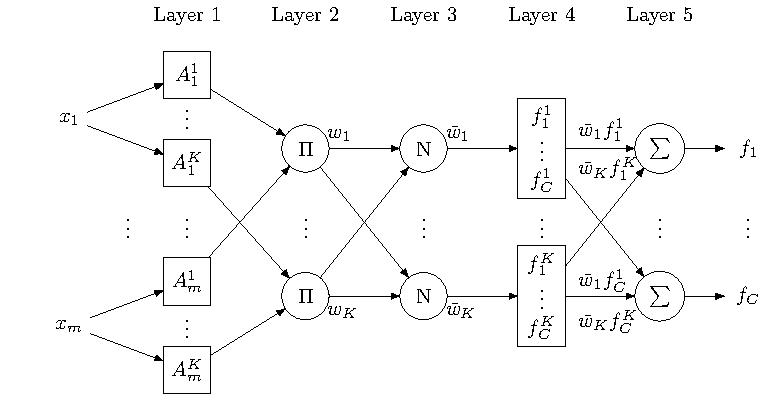
\includegraphics[width=\hsize]{anfis_architecture_classification.pdf}
\caption{\label{fig: ANFIS_architecture}多クラス分類のためのANFIS構造.}
\end{figure}

ANFIS~\cite{Jang1993}は,図\ref{fig: ANFIS_architecture}に示すように,5層のニューラルネットワークアーキテクチャによって多クラス分類のためのTS-FIS推定~\cite{Angelov2004}を実現する.
各ノードの機能は,以下のようにまとめられる.

\vspace{3mm}
\noindent
\textbf{Layer 1:}

各ノード関数は,与えられた入力$x_j$が言語ラベル$A_j^k$を満足する度合いを出力する.
ファジィメンバシップ関数は,最大値が1,最小値が0のベル型関数,またはガウス関数を用いることが一般的である.
この層でのパラメータは,「前提部パラメータ」と呼ばれ,逆伝播における勾配降下法によって更新する.

本論文では,個体$i$の$j$番目の入力$x_{ij}$の$k$番目のルールへのメンバシップ度を表現するため,前提部パラメータ$a_{kj}, b_{kj}, c_{kj}$から成る,以下で与えられるベル型関数を用いる.

\begin{equation}
	\mu_{kj} (x_{ij}) = \frac{1}{1+\left( \left(\frac{x_{ij}-c_{kj}}{a_{kj}} \right)^2 \right)^{b_{kj}}}
\end{equation}

\vspace{3mm}
\noindent
\textbf{Layer 2:}

この層の全ノードは,入力値を乗算し,その積をルール$k$の発火強度$w_{ki} = \prod_{j=1}^m \mu_{kj} (x_{ij})$として出力する.
この層では,更新すべきパラメータはない.

\vspace{3mm}
\noindent
\textbf{Layer 3:}

この層での全ノードは,すべてのルールの発火強度の和が1となるように,ルールの発火強度を正規化する.
それゆえ,個体$i$のルール$k$に対する正規化発火強度$\bar{w}_{ki}$は,発火強度$w_{ki}$を用いて,$\bar{w}_{ki} = w_{ki} / \sum_{\ell=1}^K w_{\ell i}$のように計算される.
この層においても,更新すべきパラメータはない.

\vspace{3mm}
\noindent
\textbf{Layer 4:}

各ノード関数は,各ルールの結果を以下のように出力する.

\begin{equation}
	\bar{w}_{ki} \times f_{c}^k (\bmath{x}_{i}) = \bar{w}_{ki} r_{k}^c, \quad c=1, \dots, C
\end{equation}
この層におけるパラメータ$r_{k}^c$は,「結論部パラメータ」と呼ばれ,順伝播における最小二乗推定によって更新される.

\vspace{3mm}
\noindent
\textbf{Layer 5:}

この層の$C$個のノードは,すべての入力値の総和を出力値として計算する.
つまり,各システムの出力は,以下のように与えられる$K$個のルールすべての出力のファジィメンバシップによる重み付け平均から求められる.

\begin{equation}
	\hat{y}_{ic} = f_c (\bmath{x}_{i}) = \sum_{k=1}^K \bar{w}_{ki} \times f_{c}^k (\bmath{x}_{i}), \; c=1, \dots, C
\end{equation}

また,個体$i$の出力クラス$class_i$は,次のように分類される.

\begin{equation}
	class_i = {\rm argmax}_{c} \; \hat{y}_{ic}
\end{equation}

\subsection{ノイズファジィクラスタリング}

FCM法~\cite{Bezdek81a}は,各クラスタ$k$がそのクラスタ中心$\bmath{b}_k$によって表され,クラスタ基準が入力データ$\bmath{x}_i$とクラスタ中心$\bmath{b}_k$の間のユークリッド距離によって定義される$k$個の分割をファジィに推定するためのクラスタリングアルゴリズムである.最小化すべき目的関数は,以下のように与えられる.
\begin{equation}
\begin{aligned}[b]
J_{fcm} &=\sum_{k=1}^{K} \sum_{i=1}^{n} u_{k i}^{\theta} d_{k i} \\
&=\sum_{k=1}^{K} \sum_{i=1}^{n} u_{k i}^{\theta}\left\|\bmath{x}_{i}-\bmath{b}_{k}\right\|^{2}
\end{aligned}
\label{eq: object FCM}
\end{equation}
$u_{ki}$ ($u_{ki} \in [0, 1]$)は個体$i$のクラスタ$k$へのファジィメンバシップであり,$\sum_{k=1}^K u_{ki} = 1$となるよう制約されている.
$\theta$ ($\theta > 1$)は,分割のファジィ度を調整する重み付け指数であり,$\theta$の値を大きくすると,クラスタの境界がファジィになる一方,$\theta$を1に近づけると,$k$-meansのクリスプな分割~\cite{MacQueen67}に近づく.
一般的に,$\theta = 2$がファジィ度として用いられる~\cite{Bezdek81a}.

クラスタリングアルゴリズムは,ファジィメンバシップ$u_{ki}$とクラスタ中心$\bmath{b}_k$を反復的に更新するような,交互最適化の原理に基づいて構築される.
Noise fuzzy $c$-means (NFCM)~\cite{Dave91,Dave97}は,FCM法の拡張手法であり,ノイズクラスタを追加することにより,ノイズ除去を実現している.
全個体から等しい距離$\gamma$をもつ追加のノイズクラスタのインデックスを$K+1$とする.NFCM法の目的は,以下で与えられる目的関数を最小化することによって,$K+1$個のクラスタを抽出することである.
\begin{equation}
\begin{aligned}[b]
J_{n f c m} &=\sum_{i=1}^{n}\left(\sum_{k=1}^{K} u_{k i}^{\theta} d_{k i}+u_{K+1, i}^{\theta} \gamma\right) \\
&=\sum_{i=1}^{n}\left(\sum_{k=1}^{K} u_{k i}^{\theta} \| \boldsymbol{x}_{i}-\boldsymbol{b}_{k} \|^{2}+u_{K+1, i}^{\theta} \gamma\right)
\end{aligned}
\label{eq: object NFCM}
\end{equation}
$u_{K+1, i}$は,個体$i$のノイズクラスタへのファジィメンバシップであり,メンバシップ値は以下の確率的制約の下で計算される.
\begin{equation}
	\sum_{k=1}^{K+1} u_{ki} = 1
\label{eq: sum-to-one condition for noise FCM}
\end{equation}
個体$i$が,$K$個の正常なクラスタすべてから$\gamma$以上離れている場合,その個体は,ノイズクラスタへ割り当てられ,大きなファジィメンバシップ$u_{K+1, i}$が与えられる.
そのため,$K$個の正常なクラスタのクラスタ中心をノイズの影響なしに計算できる.

ここで,正常なクラスタが1つだけであるとすると,NFCM法は,初期点をランダムにとるロバストな平均ベクトルを推定することを目的としたpossibilistic $c$-means (PCM)~\cite{Krishnapuram93}とみなすことができる.

同様の考え方が,確率的推定を用いないノイズクラスタリングに基づくロバストな分析にも応用された.
ファジィ主成分分析(Fuzzy PCA)によるロバストな$k$-means法~\cite{Honda2010_IEEE-TFS}は,個体$i$の非ノイズ度とノイズ度を表す通常のファジィメンバシップ$u_i$とその補数$1-u_i$をそれぞれ利用するようなロバストなPCAを,$k$-means法に導入しており,その目的関数は,以下の式で与えられる.

\begin{equation}
	J_{rkm} = \sum_{i=1}^n \left( (1-u_i)^\theta \gamma + u_i^\theta \sum_{k=1}^K \sum_{i \in G_k} || \bmath{x}_i - \bmath{b}_k||^2 \right)
\end{equation}

\end{document}
